%% Ryan's Latex preamble. Last updated 02/08/2021

\usepackage[utf8]{inputenc} % allow utf-8 input
\usepackage[T1]{fontenc}    % use 8-bit T1 fonts
\usepackage{booktabs}       % professional-quality tables
\usepackage{nicefrac}       % compact symbols for 1/2, etc.
\usepackage{microtype}      % microtypography

\usepackage{amssymb,amsmath,amsthm,bbm}
\usepackage[margin=1in]{geometry}
\usepackage{verbatim,float,url,dsfont}
\usepackage{graphicx,subfigure,psfrag}
\usepackage{algorithm,algorithmic}
\usepackage{mathtools,enumitem}
\usepackage[colorlinks=true,citecolor=blue,urlcolor=blue,linkcolor=blue]{hyperref}
\usepackage{multirow}
\usepackage[most]{tcolorbox}
\usepackage{zref}
\usepackage{bm}
\usepackage{ragged2e}

\DeclareMathOperator*{\argmin}{argmin}
\DeclareMathOperator*{\argmax}{argmax}
\DeclareMathOperator*{\minimize}{minimize}
\DeclareMathOperator*{\maximize}{maximize}
\DeclareMathOperator*{\find}{find}
\DeclareMathOperator{\st}{subject\,\,to}

\DeclareMathOperator{\Cov}{Cov}
\DeclareMathOperator{\Var}{Var}
\DeclareMathOperator{\dm}{dim}
\DeclareMathOperator{\col}{col}
\DeclareMathOperator{\row}{row}
\DeclareMathOperator{\nul}{null}
\DeclareMathOperator{\rank}{rank}
\DeclareMathOperator{\nuli}{nullity}
\DeclareMathOperator{\spa}{span}
\DeclareMathOperator{\sign}{sign}
\DeclareMathOperator{\supp}{supp}
\DeclareMathOperator{\diag}{diag}
\DeclareMathOperator{\aff}{aff}
\DeclareMathOperator{\conv}{conv}
\DeclareMathOperator{\dom}{dom}
\DeclareMathOperator{\tr}{tr}

\def\R{\mathbb{R}}
\def\C{\mathbb{C}}
\def\E{\mathbb{E}}
\def\P{\mathbb{P}}
\def\half{\frac{1}{2}}
\def\th{^{\text{th}}}
\def\df{\mathrm{df}}
\def\hy{\hat{y}}
\def\hf{\hat{f}}
\def\hmu{\hat{\mu}}
\def\halpha{\hat{\alpha}}
\def\hbeta{\hat{\beta}}
\def\htheta{\hat{\theta}}
\def\cA{\mathcal{A}}
\def\cB{\mathcal{B}}
\def\cD{\mathcal{D}}
\def\cE{\mathcal{E}}
\def\cF{\mathcal{F}}
\def\cG{\mathcal{G}}
\def\cK{\mathcal{K}}
\def\cH{\mathcal{H}}
\def\cI{\mathcal{I}}
\def\cL{\mathcal{L}}
\def\cM{\mathcal{M}}
\def\cN{\mathcal{N}}
\def\cP{\mathcal{P}}
\def\cS{\mathcal{S}}
\def\cT{\mathcal{T}}
\def\cW{\mathcal{W}}
\def\cX{\mathcal{X}}
\def\cY{\mathcal{Y}}
\def\cZ{\mathcal{Z}}

%% Special preamble for the book

\def\SS{\mathbb{S}} % DON'T use \S, causes errors 
\def\N{\mathbb{N}}
\def\T{\mathsf{T}}
\def\d{\mathsf{d}}
\def\pinv{{\bm{+}}}
\def\one{1}
\def\op{\mathrm{op}}
\def\TV{\mathrm{TV}}

\DeclareMathOperator{\closure}{cl}
\DeclareMathOperator{\interior}{int}
\DeclareMathOperator{\boundary}{bd}
\DeclareMathOperator{\relint}{relint}
\DeclareMathOperator{\relbd}{relbd}
\DeclareMathOperator{\epi}{epi}
\DeclareMathOperator{\ran}{ran}
\DeclareMathOperator{\cone}{cone}
\DeclareMathOperator{\prox}{prox}
\DeclareMathOperator{\vek}{vec}
\DeclareMathOperator{\infconv}{\texttt{\#}}

\newcommand{\tinyskip}{\vspace{2pt}}

% Widebar
\makeatletter
\newcommand*\rel@kern[1]{\kern#1\dimexpr\macc@kerna}
\newcommand*\widebar[1]{%
\begingroup
\def\mathaccent##1##2{%
\rel@kern{0.8}%
\overline{\rel@kern{-0.8}\macc@nucleus\rel@kern{0.2}}%
\rel@kern{-0.2}%
}%
\macc@depth\@ne
\let\math@bgroup\@empty \let\math@egroup\macc@set@skewchar
\mathsurround\z@ \frozen@everymath{\mathgroup\macc@group\relax}%
\macc@set@skewchar\relax
\let\mathaccentV\macc@nested@a
\macc@nested@a\relax111{#1}%
\endgroup
}
\makeatother

% Paragraph
\makeatletter
\renewcommand{\paragraph}{%
\@startsection{paragraph}{4}%
{\z@}{1.5ex \@plus 1ex \@minus .2ex}{-0.75em}%
{\normalfont\normalsize\bfseries}%
}
\makeatother

\setcounter{secnumdepth}{5} 
\renewcommand{\theparagraph}{\Alph{paragraph}}

\newcommand{\parlab}[1]{%
\label{#1}\localspeciallabel{#1}}

\makeatletter
\zref@newlist{specialreflist}
\zref@newprop{chapter}{\arabic{chapter}}
\zref@addprop{specialreflist}{chapter}
\zref@newprop{section}{\arabic{section}}
\zref@addprop{specialreflist}{section}
\newcommand*{\localspeciallabel}[1]{\zref@labelbylist{#1}{specialreflist}}%
\newcommand*{\parref}[1]{%
\hyperref[{#1}]{%
\zref@extractdefault{#1}{chapter}{??}.\zref@extractdefault{#1}{section}{??}.\ref*{#1}}}
\makeatother

% Theorems and friends
\newtheorem{theorem}{Theorem}[chapter]
\newtheorem{lemma}[theorem]{Lemma}
\newtheorem{corollary}[theorem]{Corollary}
\theoremstyle{definition}
\newtheorem{definition}[theorem]{Definition}
\newtheorem{example}[theorem]{Example}
\newtheorem{exercise}[theorem]{Exercise}
\theoremstyle{remark}
\newtheorem{remark}[theorem]{Remark}

\newenvironment{Example}
{\smallskip
\begin{tcolorbox}[enhanced,breakable,colback=red!5!white,colframe=red!75!black]
\begin{example}}
{\end{example}
\end{tcolorbox}
\smallskip}

\newenvironment{Theorem}[1][]
{\smallskip
\begin{tcolorbox}[enhanced,breakable,colback=blue!5!white,colframe=blue!75!black]
\begin{theorem}[#1]}
{\end{theorem}
\end{tcolorbox}
\smallskip}

\newenvironment{Lemma}[1][]
{\smallskip
\begin{tcolorbox}[enhanced,breakable,colback=blue!5!white,colframe=blue!75!black] 
\begin{lemma}[#1]}
{\end{lemma}
\end{tcolorbox}
\smallskip}

\newenvironment{Corollary}[1][]
{\smallskip
\begin{tcolorbox}[enhanced,breakable,colback=blue!5!white,colframe=blue!75!black] 
\begin{corollary}[#1]}
{\end{corollary}
\end{tcolorbox}
\smallskip}

\newenvironment{Remark}[1][]
{\smallskip
\begin{tcolorbox}[enhanced,breakable,colback=gray!5!white,colframe=gray!75!black]
\begin{remark}[#1]}
{\end{remark}
\end{tcolorbox}
\smallskip}

% Less horizontal space for lists
\setlist[itemize]{leftmargin=1cm}
\setlist[enumerate]{leftmargin=1cm}

% Title page
\newcommand{\coverpic}{
\begin{minipage}{0.7\textwidth}
\vspace*{1cm}\centering
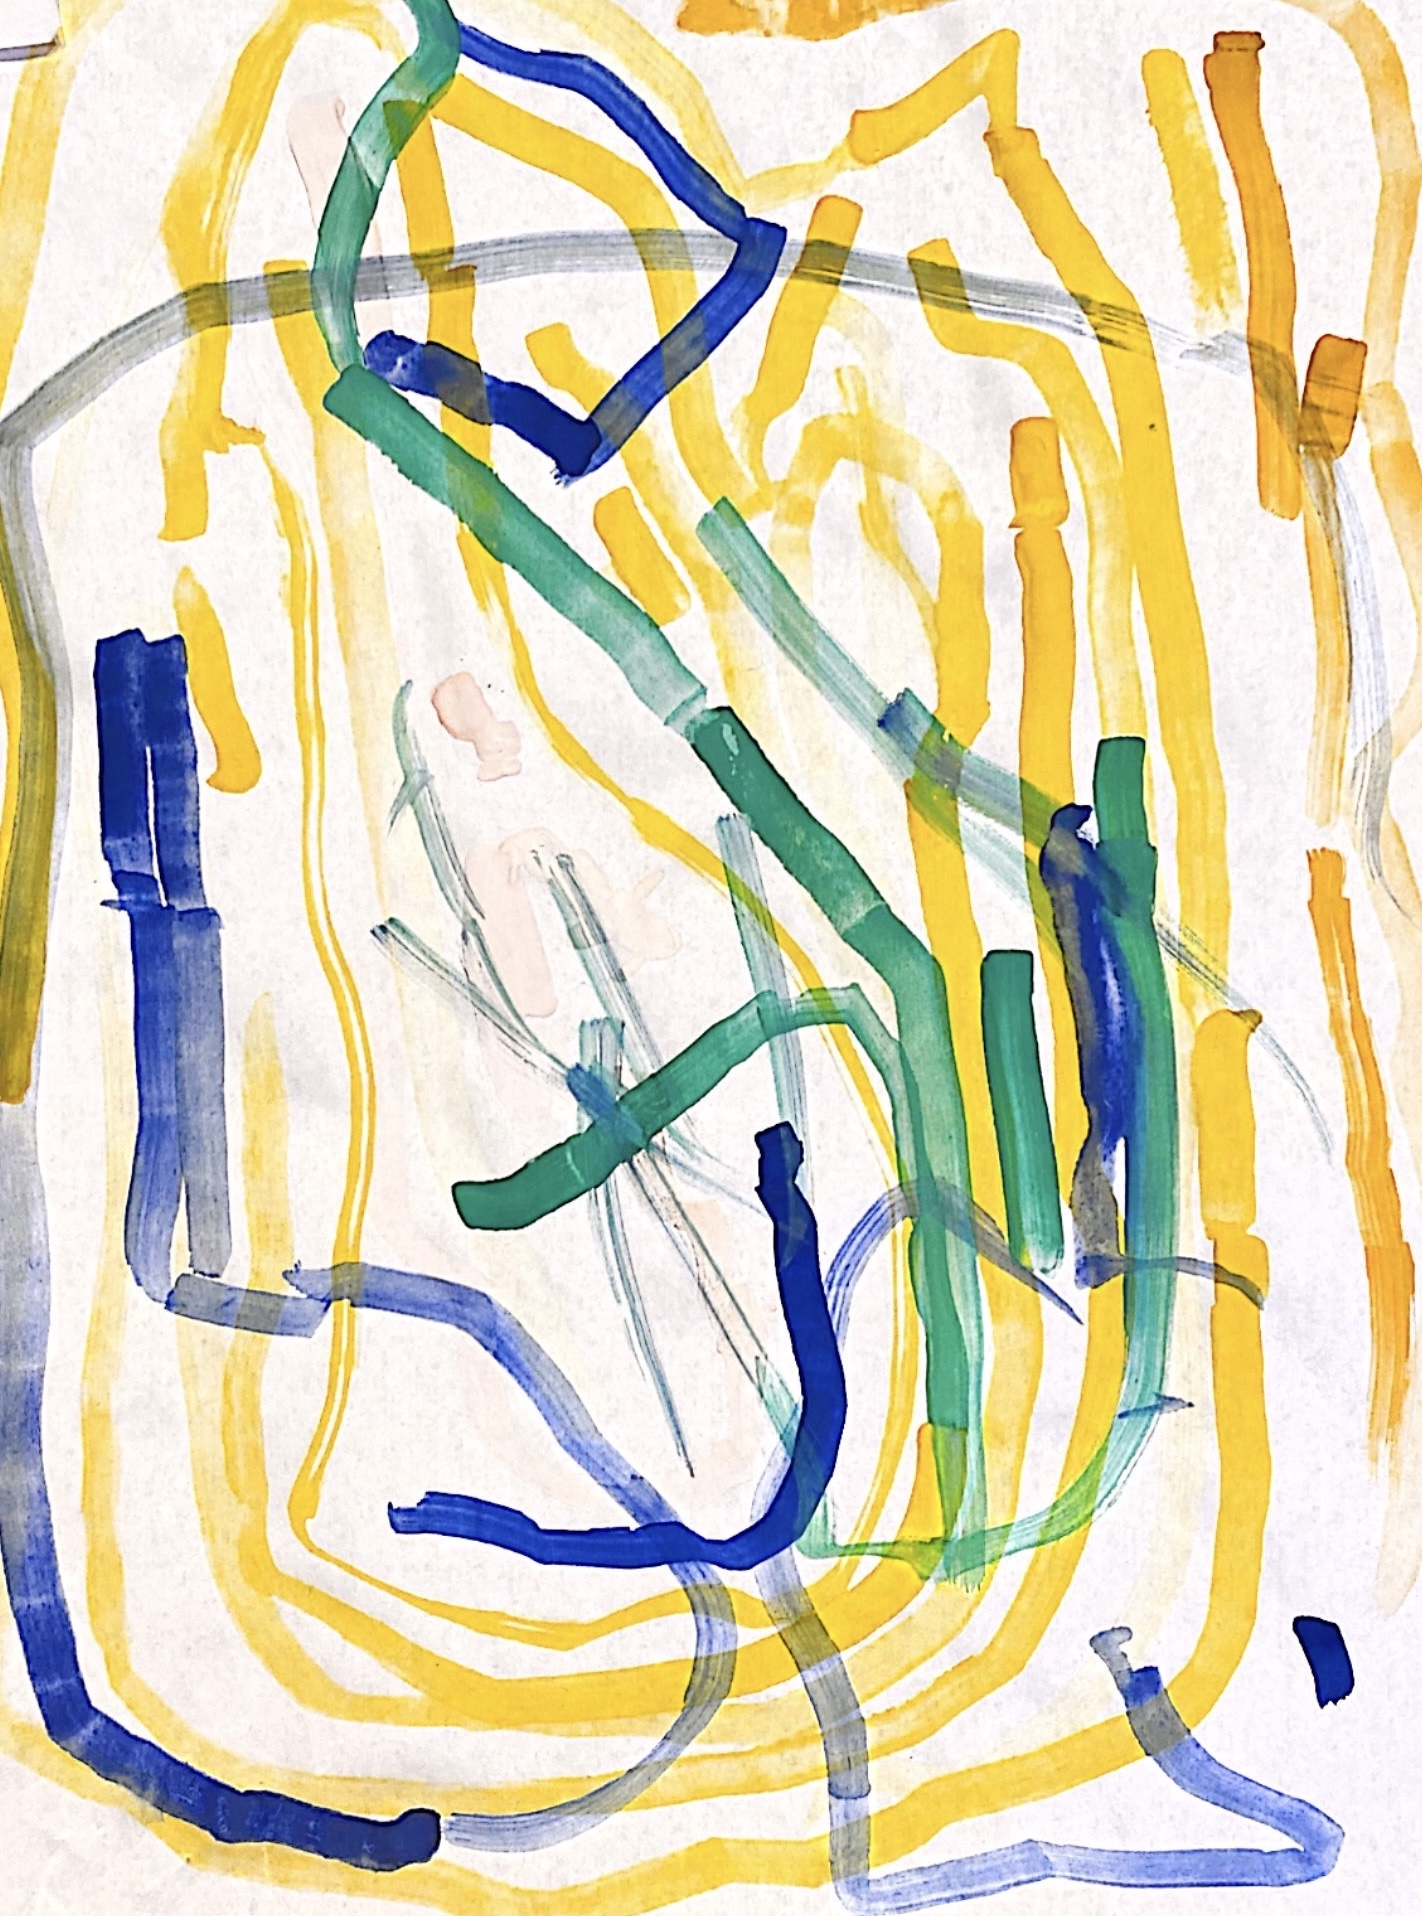
\includegraphics[width=\textwidth]{cover.jpg}
\vspace{1cm}
\end{minipage}
\par
}
\makeatletter
\renewcommand{\@maketitle}{%
\thispagestyle{plain}%
\begingroup \topskip\z@skip
\null\vfil
\centering
\begingroup
\Huge\bfseries
\@title\par\vspace{24pt}%
\def\and{\par\medskip}\centering
\Large\mdseries\authors\par\bigskip
\endgroup
\vfil
\coverpic
\vspace{10cm}
\endgroup
\newpage
}
\makeatother

% Skip entry in TOC 
\DeclareRobustCommand{\gobblefive}[5]{}
\newcommand*{\SkipTocEntry}{\addtocontents{toc}{\gobblefive}}

% % Inkscape figures
% \usepackage{import,xifthen,pdfpages,transparent}

% \newcommand{\incfig}[2]{%
% \def\svgwidth{#2}
% \import{./fig/}{#1.pdf_tex}
% }
